\subsection{Enkät}
Enkäten besvarades av 172 personer. En majoritet av de svarande föredrar en väckarklocka som visar datum men inte sekunder. Den mest önskade färgen för väckarklockans skal är svart. För fullständiga svar, se \hyperref[sec:svar]{bilaga 6.1}.

%\subsection{Önskade funktioner}
%slå kansek ihop med punkt efter

\subsection{Prototyp}
    Prototypen av väckarklockan grundades på enkortsdatorn Raspberry~Pi~3. Kopplingen kopplades på ett kopplingsdäck. Information visas på en LCD-skärm som kan visa 32 tecken fördelade på två rader. Tre knappar är kopplade till datorn vilket motsvarar $+$, $-$ och $\triangleright$. Andra komponenter är en extern högtalare, potientiometrar för att justera displayens ljusstyrka, resistorer och kablar. Se figur 1 för kopplingen av prototypen och figur 2 för ett kopplingschema över kretsen. För större schema, se \hyperref[sec:krets]{bilaga 6.2}.
    \begin{figure}[h!]
    \centering

        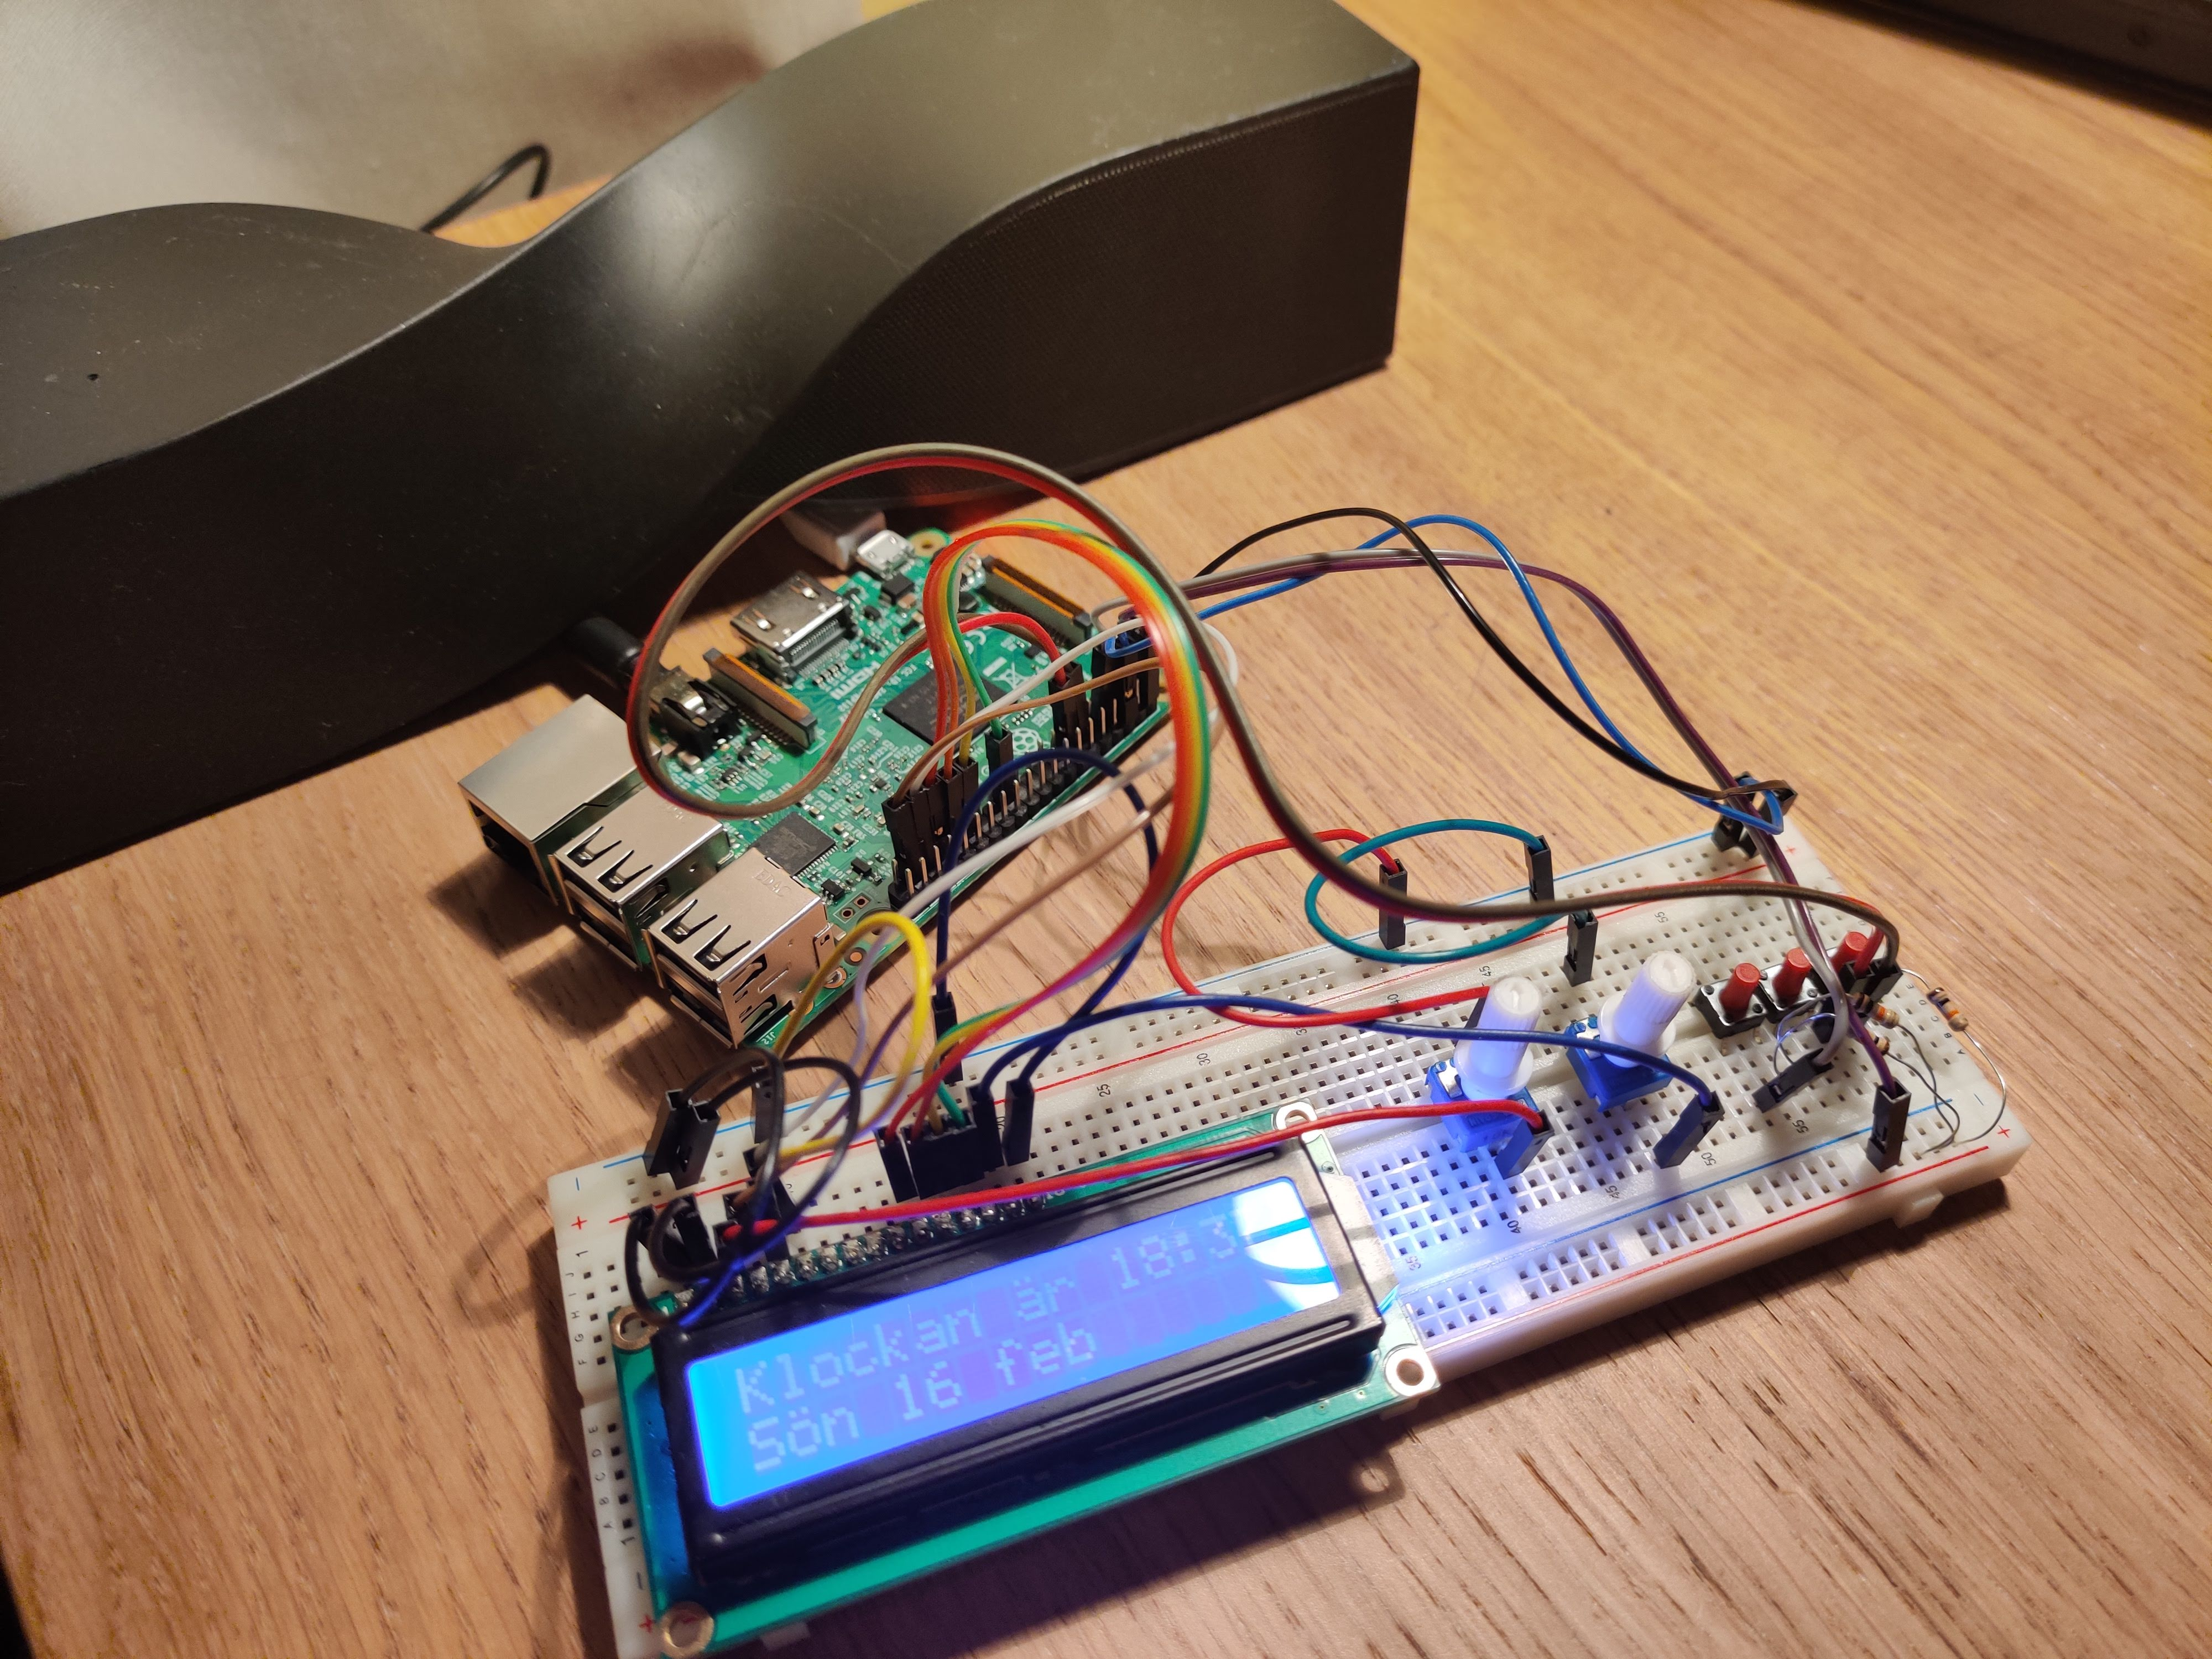
\includegraphics[width=0.4\textwidth]{bilder/koppling.jpg} % first figure itself
        \caption{Kopplingen av protoypen}
    \end{figure}
    \begin{figure}[h!]
    \centering
        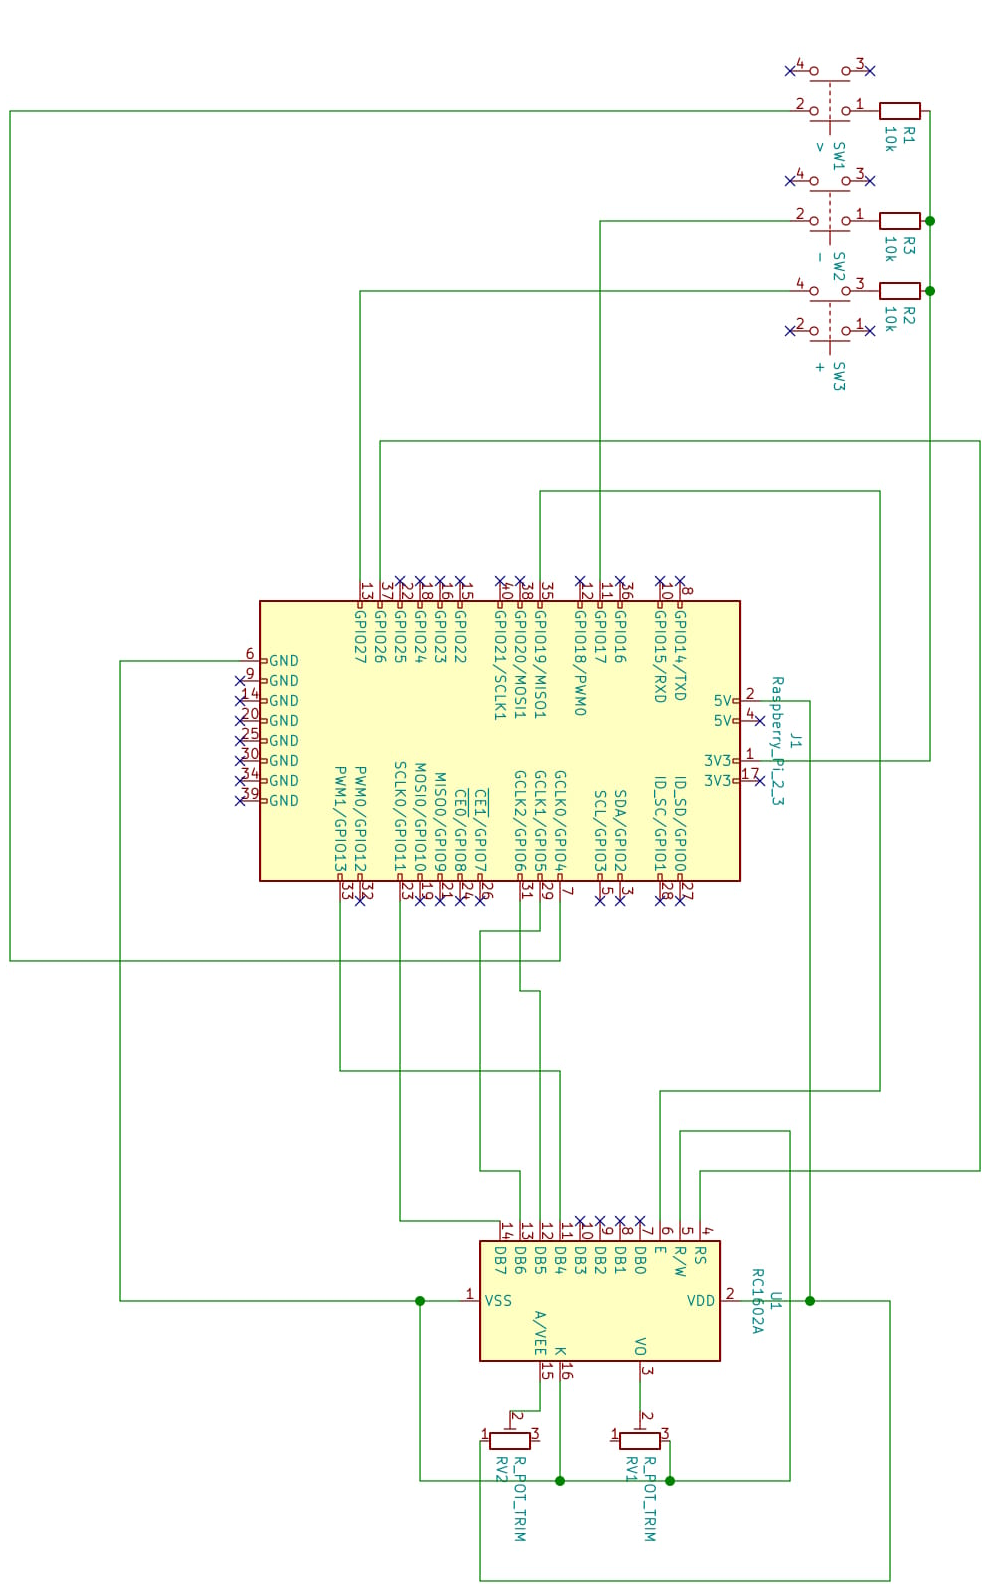
\includegraphics[width=0.35\textwidth,angle=90]{bilder/krets2.png} % second figure itself
        \caption{Kopplingschema}
    \end{figure}

\subsection{Program}
Programmet för väckarklockan är skrivet i programmeringsspråket \emph{Python} version 2.7 och LCD-bibliotek \texttt{CHARLcd} ligger som grund för användar\-kommunikation. Väckarklockans program låter användaren ställa in önskad alarmtid (figur 3) och därefter välja ifall alarmet ska ringa eller inte. När alarmet ringer spelas ljud från en ljudfil upp på repetition tills användaren svarar rätt på en fråga. 

När $\triangleright$ trycks in anropas metoden \verb|alarmvisning| och den tidigare inställda alarmtiden visas. Först ställs timmarna in och därefter minuterna. Alarmtiden kan ställas in i intervall om fem minuter. 

För att  inte tiden ska kunna understiga 00:00 respektive överstiga 23:55 används 
\small{\mint{python}|if (GPIO.input(13) == GPIO.HIGH and alarmH<23 and raknareAlarm==0):| }
\normalsize \noindent och andra liknande if-satser. Variabeln \verb|raknareAlarm| håller reda på ifall det är timmarna eller minuterna som ska ställas in. Ifall \verb|raknareAlarm| är 0 ställs timmarna in, vid 1 ställs minuterna. 

Varje minut uppdateras skärmen med den nya tiden. Detta sker genom att varje gång \mintinline{python}{time.strftime("\%S")} (hämtning av sekunderna) är lika med 0 anropas metoden \texttt{tidsvisning}. 
\begin{minted}[fontsize=\footnotesize]{python}
def tidsvisning():
    lcd.cursor_mode="hide"
    lcd.clear()
    lcd.cursor_pos = (0,0)
    lcd.write_string("Klockan %sr %s" %(unichr(1), time.strftime("%H:%M")))
    lcd.cursor_pos = (1, 0)
    lcd.write_string(dag + "%s" %time.strftime(" %d ")+ man.lower() )
    if (alarmPa):
        lcd.cursor_pos=(1,15)
        lcd.write_string(unichr(3))
    time.sleep(.7)
    \end{minted}
Metoden skriver ut nuvarande tid, dag och datum. Om alarmet är aktiverat visas även en symbol för detta.

Initiering av larmet fungerar på ett liknande sätt som initieringen av tidsvisningen. Skillnaden är att den nuvarande tiden nu jämförs med den inställda alarmtiden. Om det stämmer samt att variabeln \texttt{alarmPa} är sann spelas alarmljudet upp på repetition med hjälp av biblioteket \texttt{pygame}. Samtidigt som detta sker slumpas ett tal fram mellan ett och tolv. Detta bestämmer vad för frågetyp som kommer visas, boolesk eller matematisk. Om det framslumpade talet är under fyra kommer en boolesk fråga visas, annars en matematisk fråga. 


%Den andra typen av fråga är booleska. Denna typ av fråga är ett påståen\-de och användaren får svara ifall påståendet är sant eller falskt (figur 5). 



Ifall det blir en boolesk fråga (figur 4) väljs en fråga från textdokumentet \hyperref[sec:fragor]{\texttt{fragor.txt}} (bilaga 6.4) och skrivs ut på skärmen. För att besvara frågan trycker användaren på korresponderande knapp till sant eller falskt. Därefter kontrolleras det ifall inmatningen är korrekt och då stängs alarmet av annars ändras frågan till en ny. 

Om det blir en matematisk fråga (figur 5) istället körs nedanstående kod.
\begin{minted}[fontsize=\footnotesize]{python}
a = random.randint(0,12)
b = random.randint(0,12)
c = random.randint(0,50)
svar= a*b+c
svarAnvandare= svar + random.randint(-30,30)
lcd.cursor_mode = "blink"
\end{minted}
Först slumpas tre olika variabler och svaret räknas ut. För att det ska bli färre tryck och lättare för användaren sätts grundsvaret i intervallet $\pm 30$. Användaren får sedan använda knapparna för att höja eller sänka grundsvaret. När den tror att det är rätt trycker den på $\triangleright$. Ifall det inmatade svaret är korrekt stängs alarmet av, annars får den en ny chans.


%Två typer av frågor, slumpar. Ställa in alarm intervall 
% av att ta inmatning från användaren med hjälp av tre knappar. Användaren kan ställa in alarmet själv i fem minuters intervaller och sätta på det. Alarmet

För koden, se \hyperref[sec:kod]{bilaga 6.4}. 


\begin{figure}[h!] %se till att det är på samma sida
    \centering
    \begin{minipage}{0.30\textwidth}
        \centering
        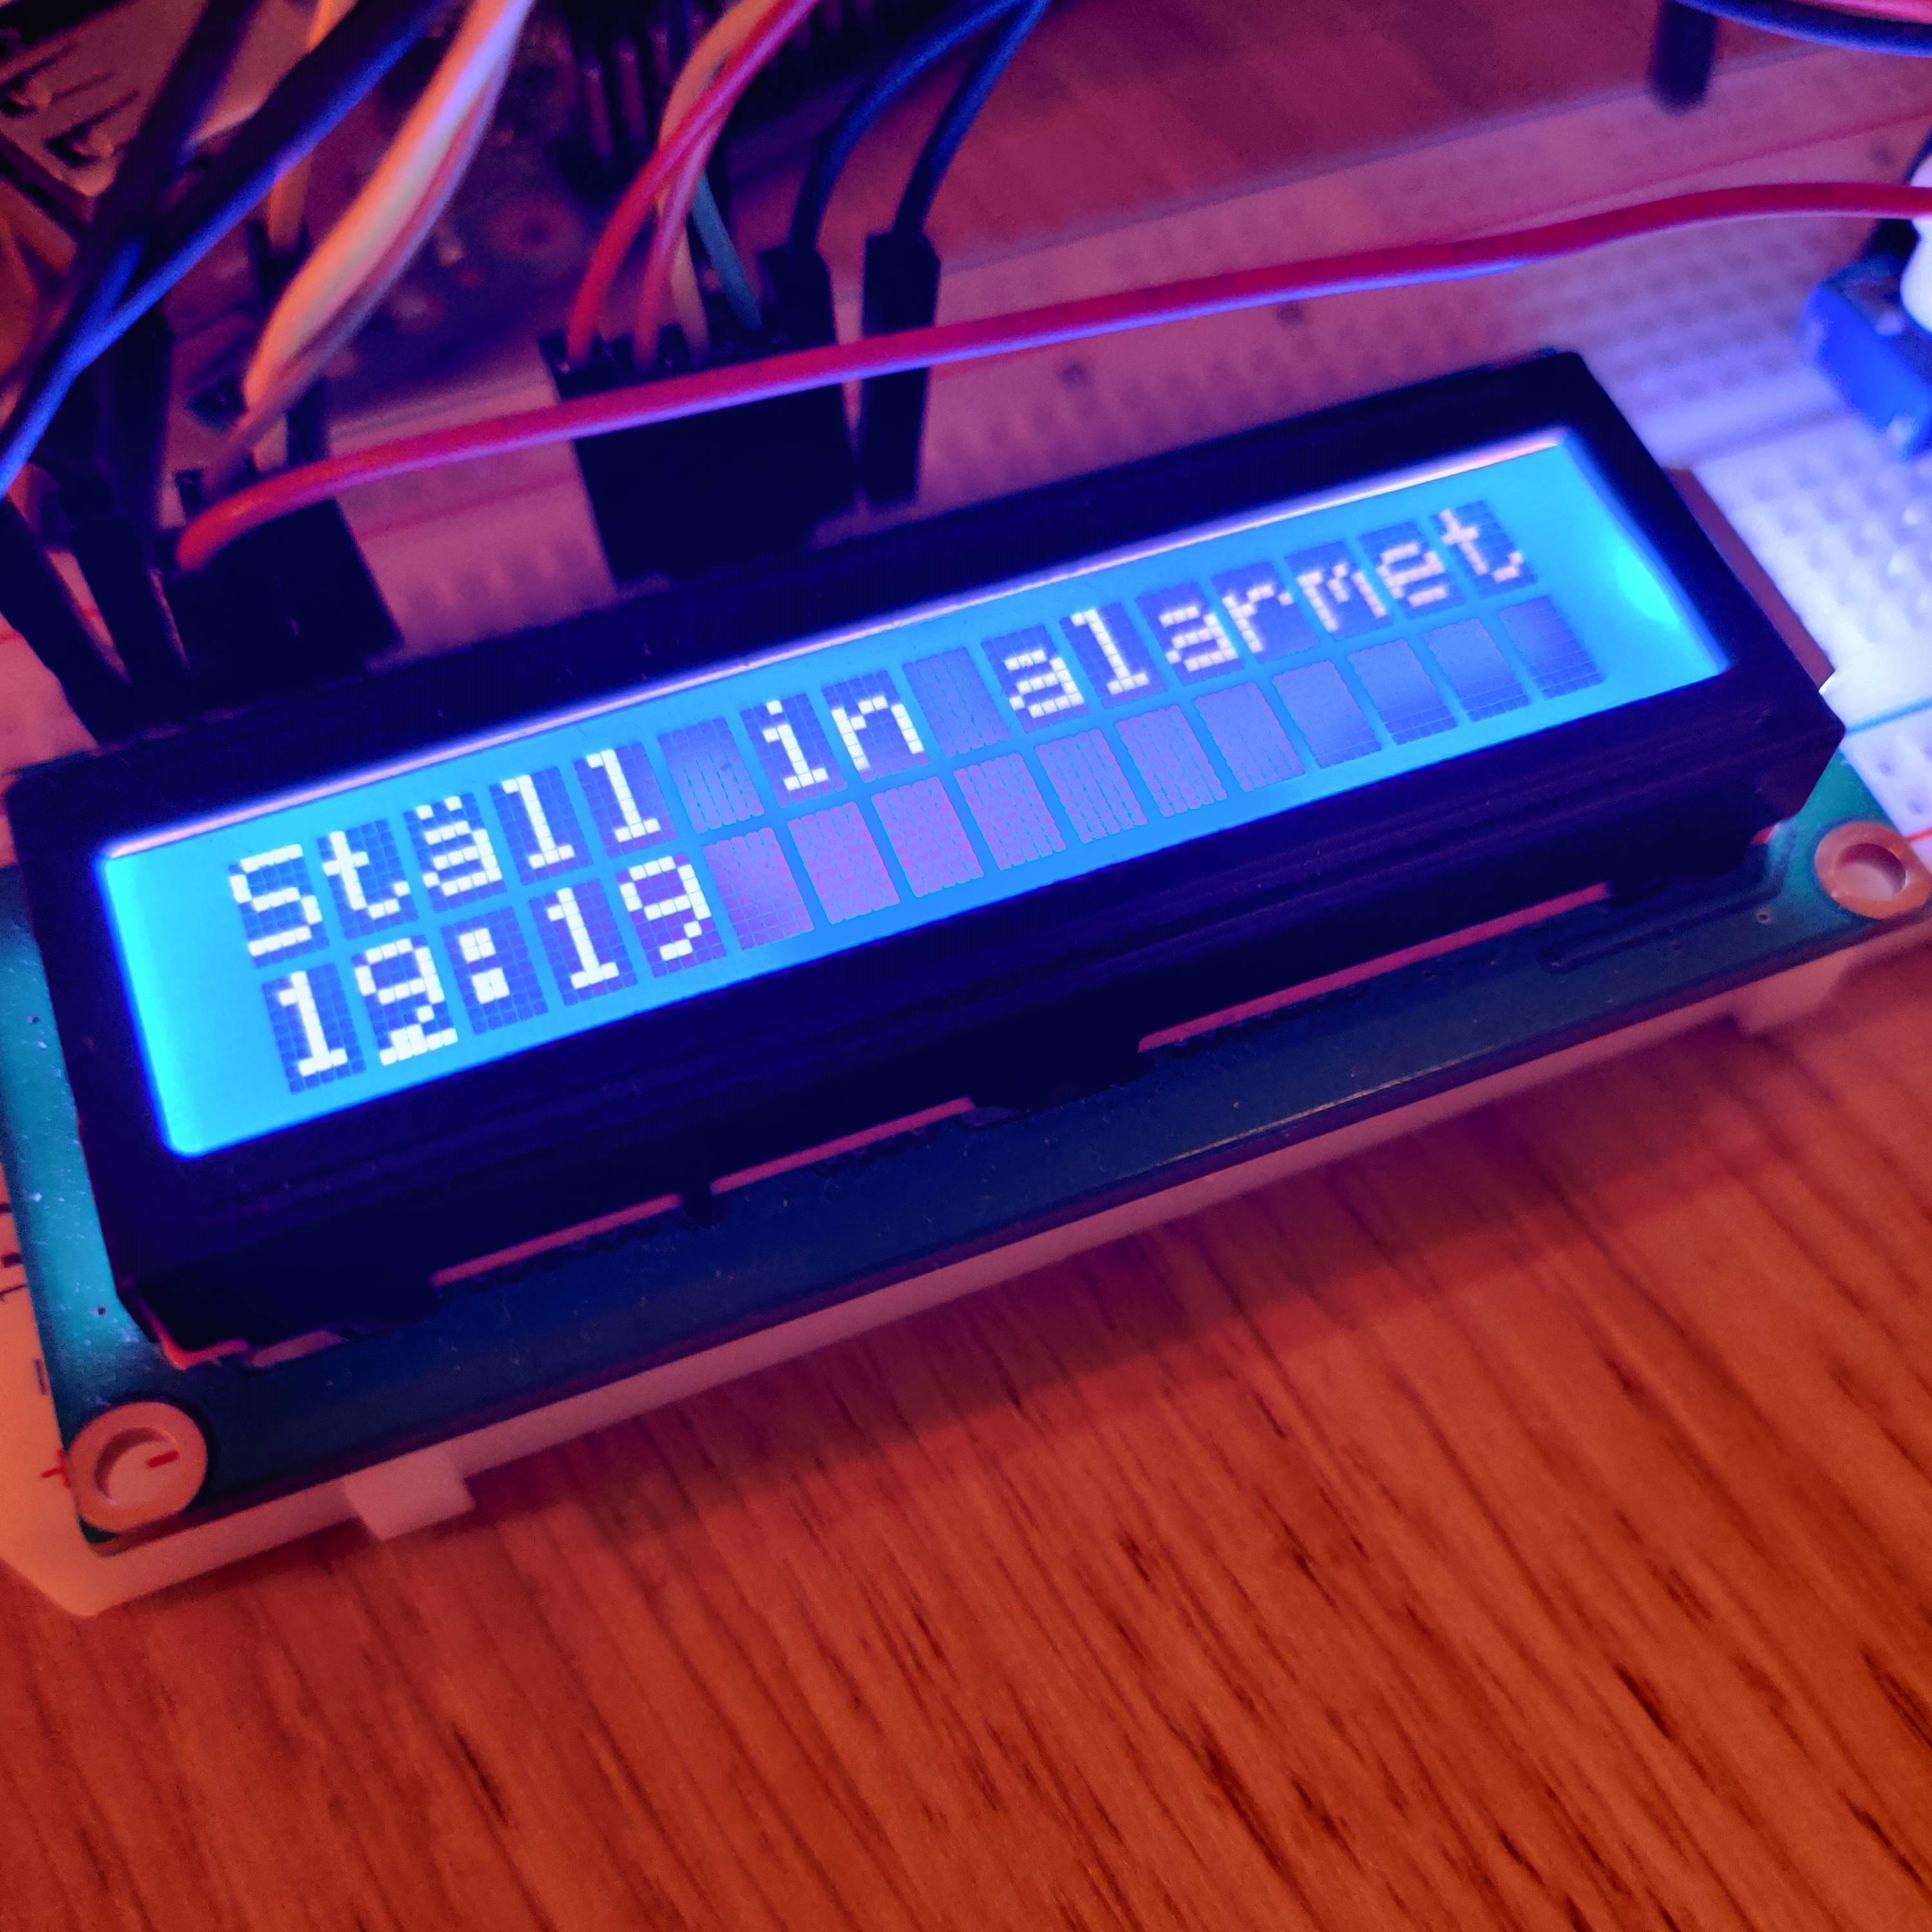
\includegraphics[width=0.9\textwidth]{bilder/stall alarm.jpg} % first figure itself
        \caption{Displayen vid inställning av alarmtid}
    \end{minipage}\hfill
    \begin{minipage}{0.30\textwidth}
        \centering
        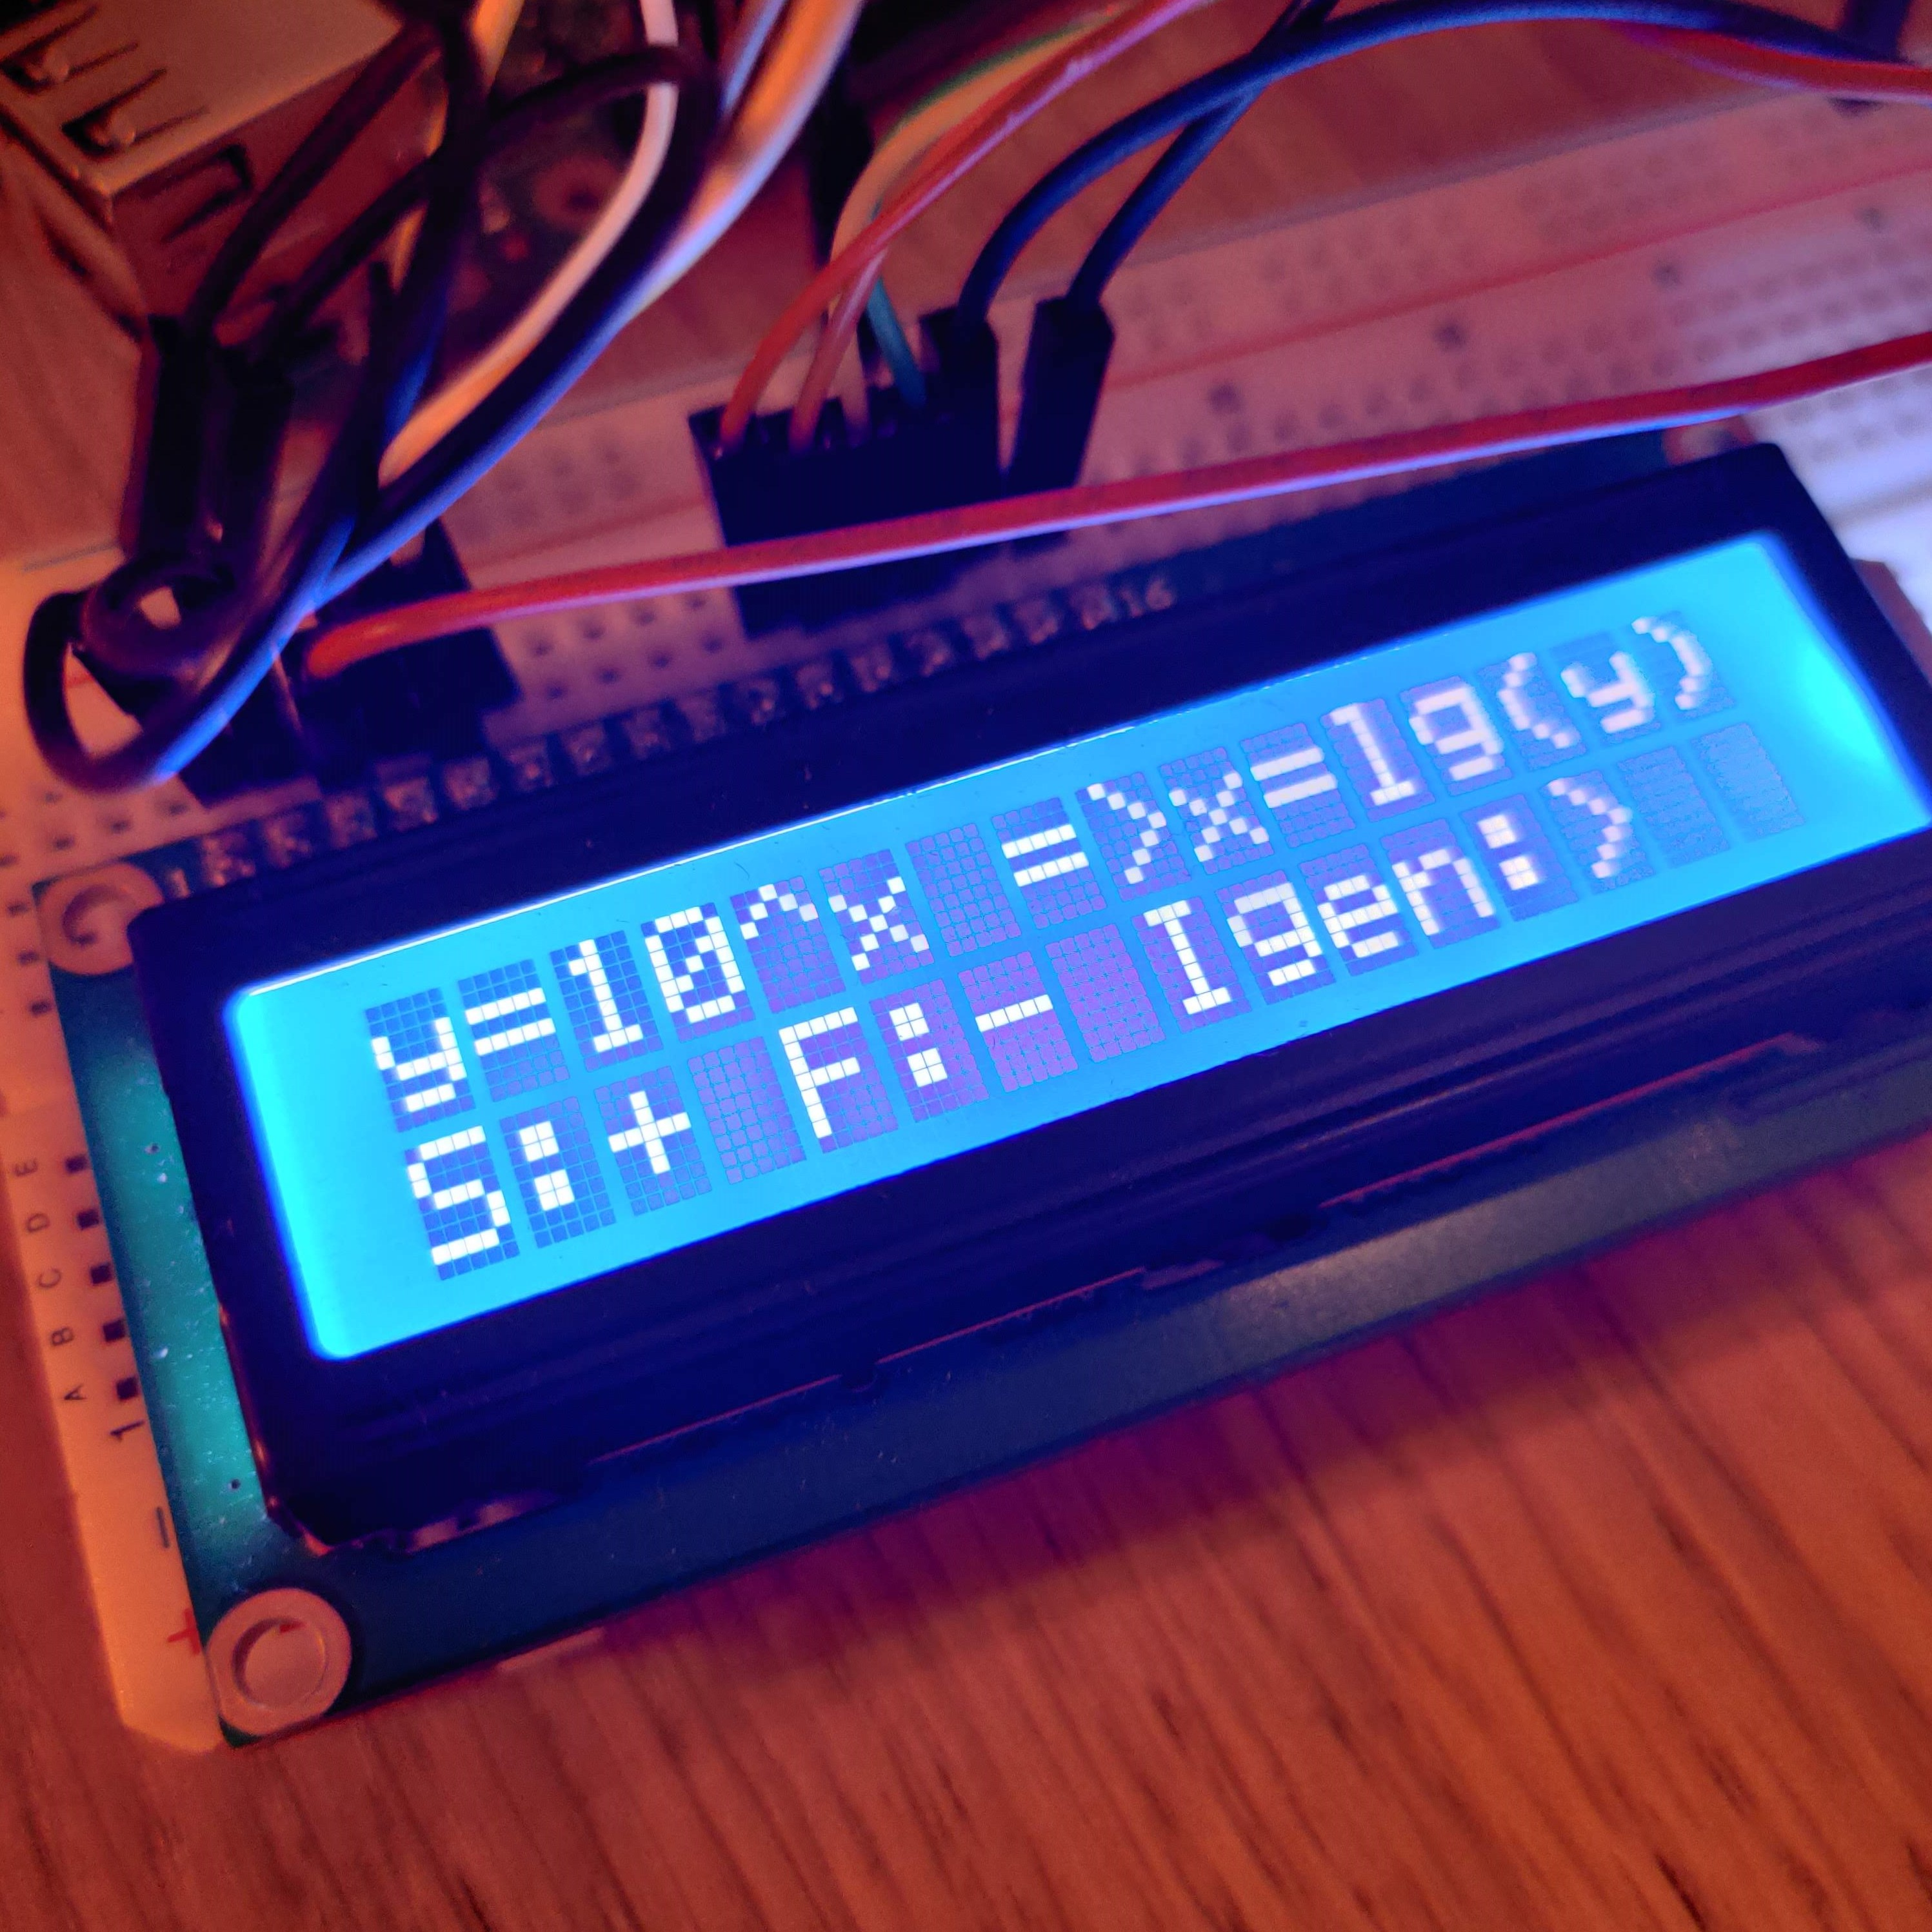
\includegraphics[width=0.9\textwidth]{bilder/sf fraga.jpg} % second figure itself
        \caption{En boolesk fråga}
    \end{minipage}\hfill
    \begin{minipage}{0.30\textwidth}
        \centering
        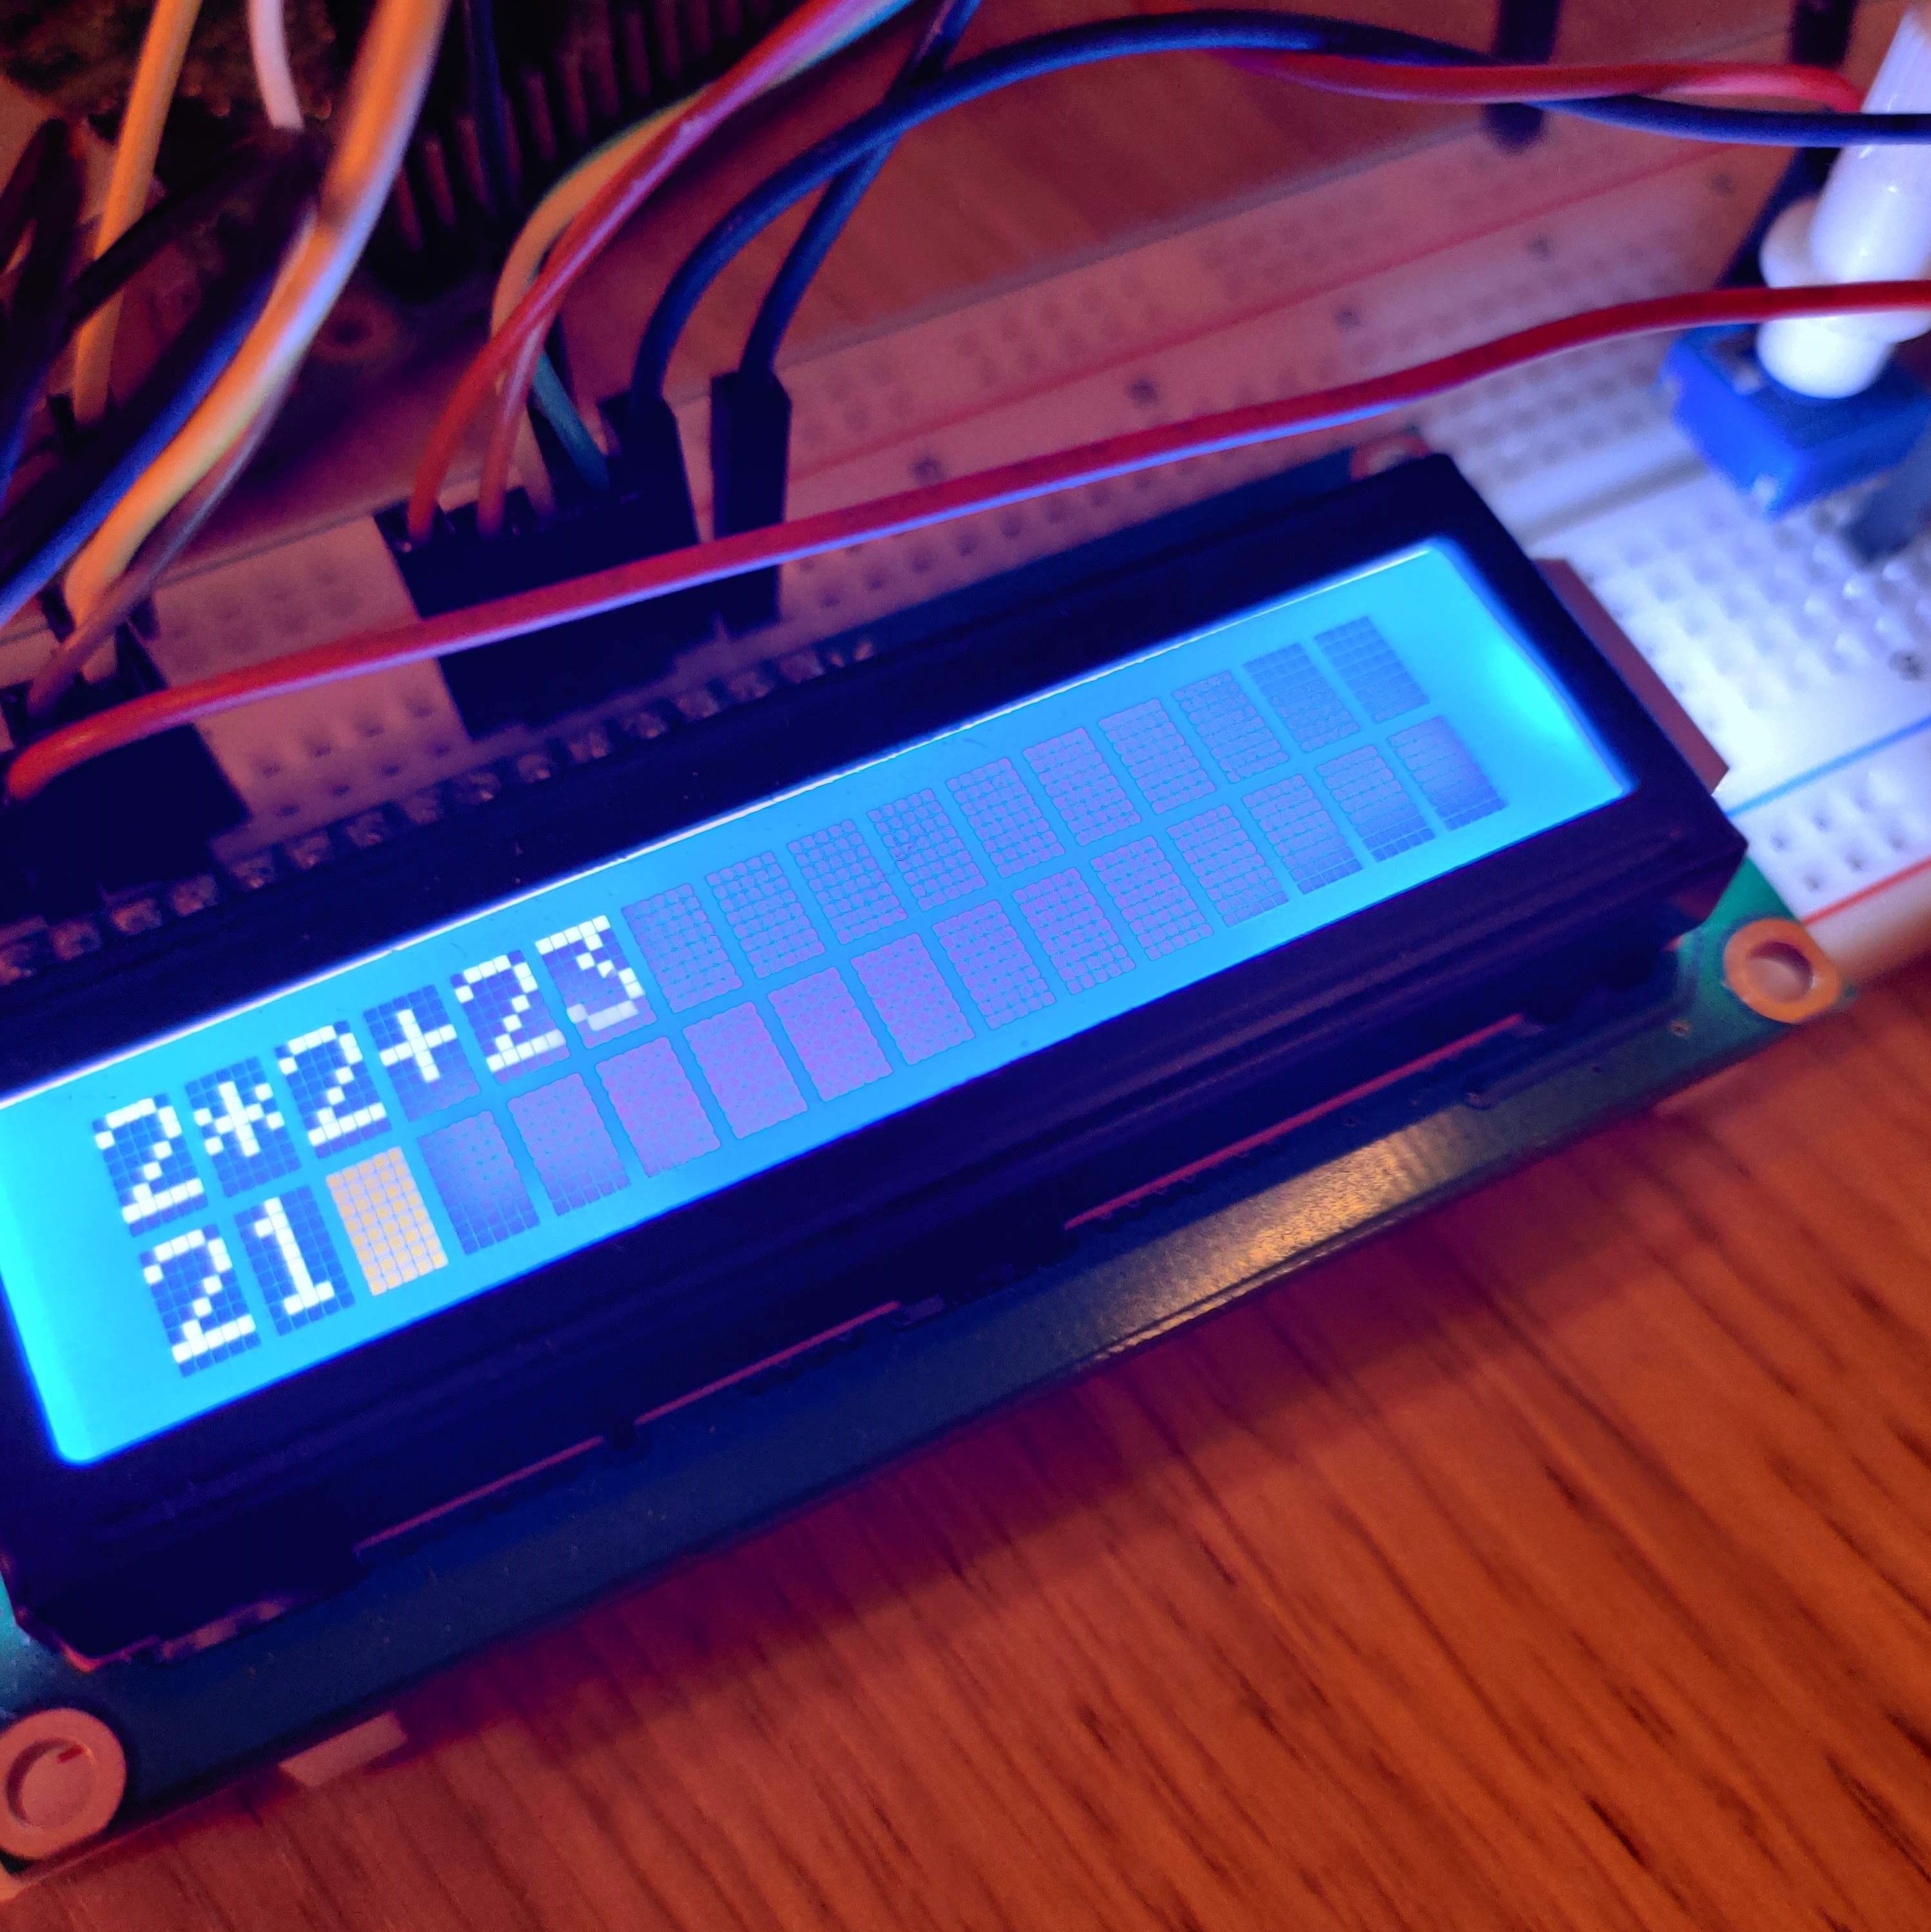
\includegraphics[width=0.9\textwidth]{bilder/ma alarm.jpg} % second figure itself
        \caption{En matematisk fråga}
    \end{minipage}
\end{figure}

%skrivet i python. Viktgia avsnitt bilder på skärmen för den kodbiten
%\subsection{Test}

